\chapter{Desenvolvimento}
\label{chapter:desenvolvimento}

Este capítulo descreve a arquitetura e a implementação do \textit{G-FShield}. A contribuição apresentada aqui é arquitetural e de engenharia de software: integrar a construção de soluções iniciais, o refinamento por busca local, a mensageria, a persistência e a inspeção operacional. Os algoritmos de seleção e de busca empregados derivam de trabalhos anteriores e não são reivindicados como novos.

\section{Visão Geral e Contrato de Entrada}

O \textit{G-FShield} foi estruturado em três camadas: uma camada web de operação, uma camada de orquestração e persistência e uma camada de execução distribuída. A primeira apresenta o estado observado e recebe comandos; a segunda concentra a \ac{api}, o banco de dados, o \textit{cache} e a integração com a mensageria; a terceira executa a geração distribuída da lista restrita de candidatos (\ac{drg}) e a busca local distribuída (\ac{dls}). A Figura~\ref{fig:arquitetura-resumo} sintetiza essas fronteiras.

\begin{landscape}
\begin{figure}[p]
  \centering
  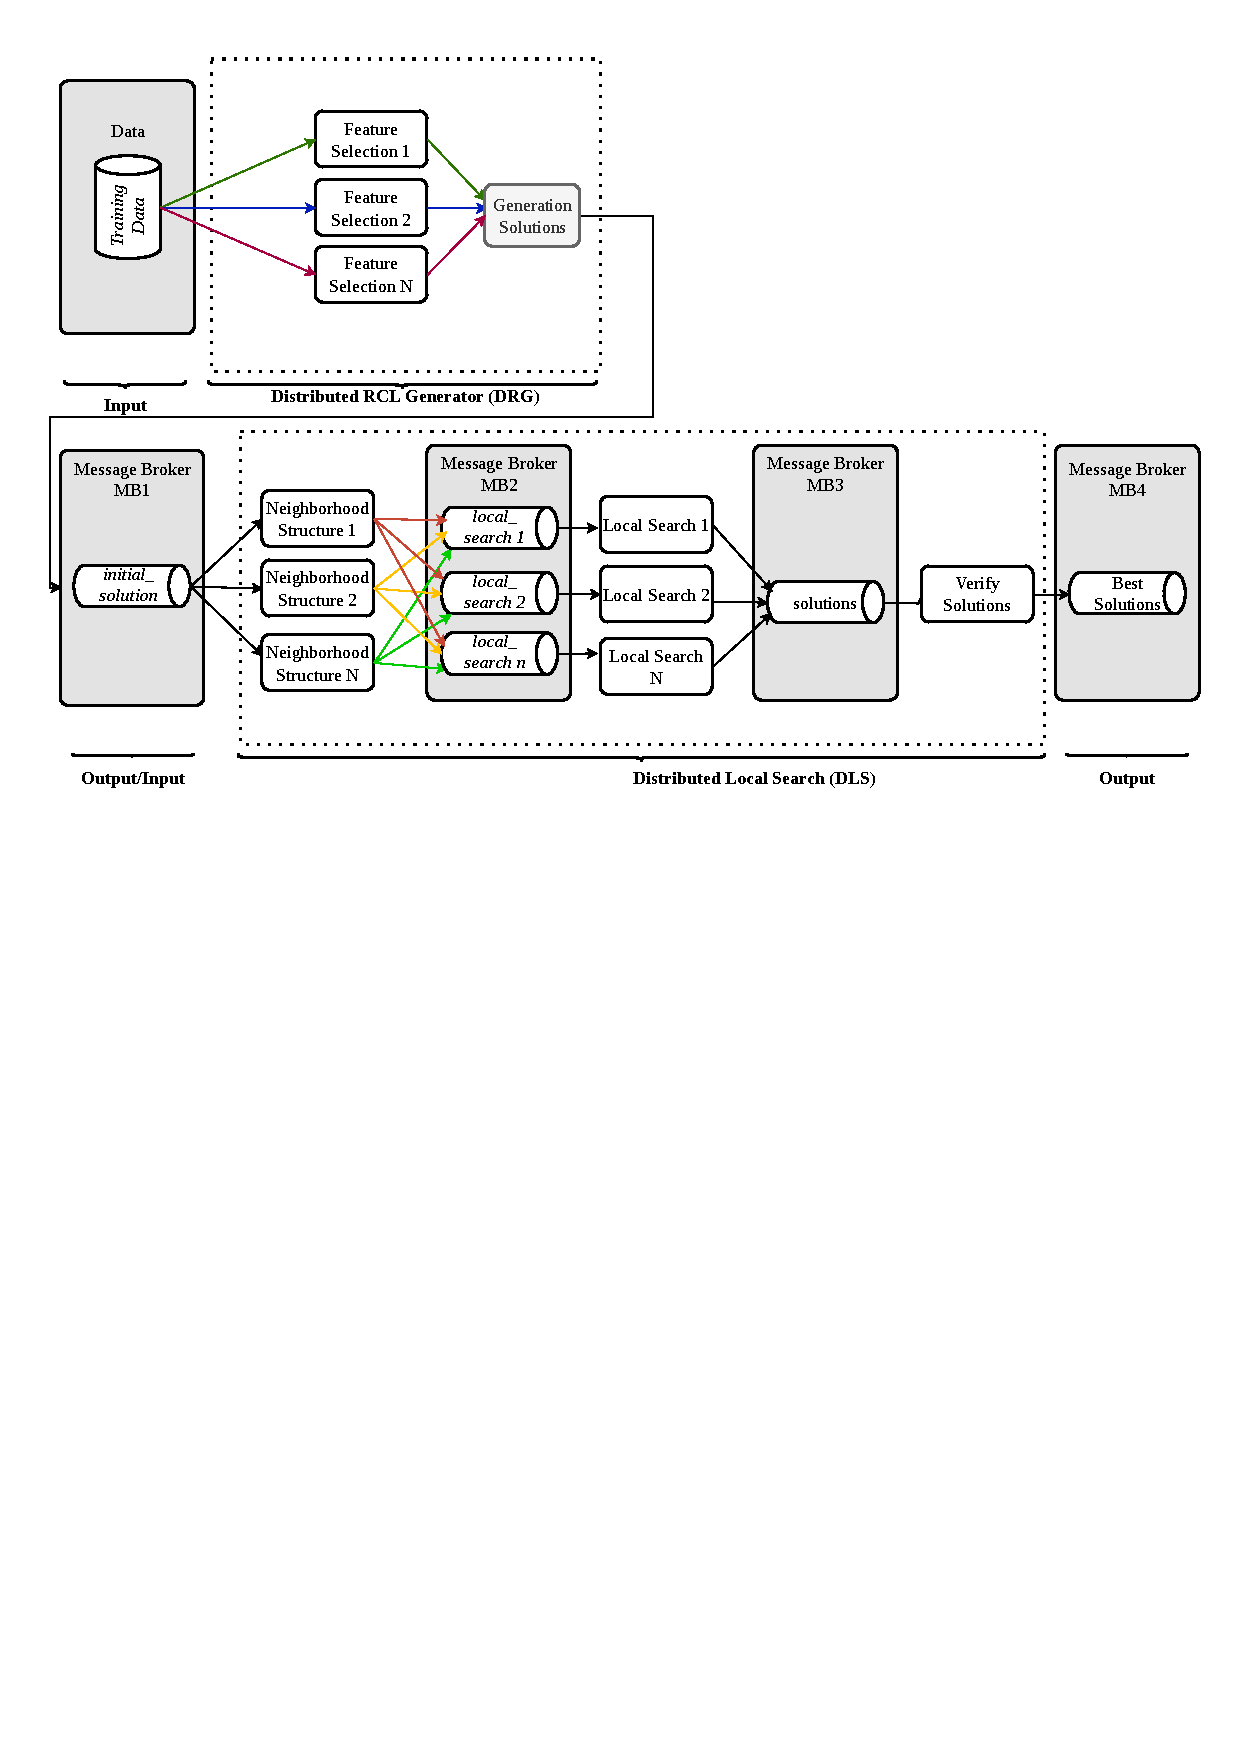
\includegraphics[trim=0 420bp 0 0,clip,width=.96\linewidth,height=.82\textheight,keepaspectratio]{fig/gfshield/arquitetura-full-summary.pdf}
  \caption{Resumo da arquitetura do \textit{G-FShield}; a margem em branco do arquivo original foi removida somente na inclusão LaTeX.}
  \label{fig:arquitetura-resumo}
\end{figure}
\end{landscape}

A independência em relação à fonte dos dados é condicionada a um contrato concreto. A API algorítmica recebe dois arquivos ARFF distintos, um de treino e outro usado para pontuar candidatos, acessíveis em \texttt{/datasets}. Ambos devem possuir o mesmo esquema e rótulo no último atributo. Na campanha formal, o segundo arquivo é a validação; o teste reservado é acessado somente pelo avaliador final. O leitor Weka define o último atributo como classe, e os preditores são identificados a partir de um. Os classificadores aceitos pela aplicação são J48, Naive Bayes e Random Forest; a campanha fixa J48.

Consequentemente, tráfego, protocolos ou \textit{logs} não são consumidos em formato bruto: precisam ser previamente transformados em matrizes rotuladas que satisfaçam esse contrato. A generalidade, portanto, é arquitetural e de formato de entrada, não evidência empírica de desempenho em fontes heterogêneas. Os CSVs históricos referenciam \texttt{erenoall.arff}, enquanto o script atual usa a separação ERENO~1k; sem manifesto, não se atribui uma configuração à outra. No \texttt{erenoall.arff} disponível, \textit{grayhole} ocupa o índice zero e \textit{normal} o índice um. Embora o nome \texttt{normalClass=0} permaneça em rotinas binárias legadas, esse caminho foi desabilitado antes da construção das imagens da campanha formal; a avaliação ativa percorre as nove classes do ARFF e calcula F1 macro.

Cada requisição informa os arquivos de treino e teste, o classificador, o número de gerações, o corte da RCL, o tamanho da amostra inicial, a estratégia VND ou RVND, as buscas locais habilitadas e, opcionalmente, limites de iteração. Esses campos formam a unidade de configuração propagada entre os serviços. Cada solução recebe ainda um \texttt{seedId} aleatório, usado para correlacionar os refinamentos que dela derivam.

\section{Drivers e Decisões Arquiteturais}

A decomposição foi orientada por seis drivers: vazão, desacoplamento, rastreabilidade, persistência, inspeção de resultados intermediários e possibilidade de evolução operacional. A Tabela~\ref{tab:architecture-drivers} explicita a relação entre esses drivers e as decisões adotadas. A decomposição em serviços e a comunicação assíncrona seguem princípios usuais de sistemas distribuídos e arquiteturas de microserviços~\cite{Tanenbaum2007Distributed,Newman2021,Kreps2011}.

\begin{table}[!htb]
  \centering
  \small
  \caption{Drivers, decisões e limites da arquitetura.}
  \label{tab:architecture-drivers}
  \begin{tabularx}{\linewidth}{@{}p{.18\linewidth}X X@{}}
    \toprule
    \textbf{Driver} & \textbf{Decisão de projeto} & \textbf{Escopo da evidência} \\
    \midrule
    Vazão & Executar os quatro rankings em serviços independentes e encaminhar sementes a operadores de busca desacoplados. & A avaliação mede a configuração implantada; não demonstra eficiência sob recursos iguais. \\
    Desacoplamento & Usar tópicos Kafka entre construção, controladores, operadores, verificador e monitor. & O acoplamento temporal é reduzido, mas a robustez diante de falhas não foi experimentalmente medida. \\
    Rastreabilidade & Propagar \texttt{seedId}, algoritmo, busca, iterações, conjuntos de atributos e métricas. & Reconstrói-se a sequência observada pelo monitor, não uma prova de completude do fluxo. \\
    Persistência & Armazenar lançamentos, execuções, eventos e agregados no PostgreSQL e CSVs no volume de métricas. & Redis é \textit{cache}; não substitui o armazenamento persistente. \\
    Inspeção intermediária & Publicar progresso selecionado, soluções refinadas e melhores soluções observadas. & A interface apresenta telemetria; ela não torna o algoritmo explicável. \\
    Evolução operacional & Isolar responsabilidades para permitir replicação e substituição por serviço. & Escalabilidade e tolerância a falhas são objetivos de projeto, não resultados demonstrados. \\
    \bottomrule
  \end{tabularx}
\end{table}


As fases de construção e refinamento possuem custos e padrões de consumo diferentes. Por isso, foram separadas em serviços com limites próprios de CPU, memória e concorrência. Essa separação permite observar e alterar uma responsabilidade sem incorporar toda a busca em um único processo. Ela também torna possível aumentar o número de instâncias de um serviço; contudo, a relação entre réplicas, vazão e custo precisa de um experimento de escala específico.

A persistência e o histórico de eventos foram adotados para reduzir a dependência de estado mantido apenas em memória. A configuração avaliada, entretanto, usa um único \textit{broker} Kafka e fator de replicação um. Assim, não se infere alta disponibilidade ou tolerância a falhas a partir da decomposição. Essas propriedades exigiriam injeção de falhas, verificação de reentrega, idempotência, recuperação e reprocessamento.

\section{Geração Distribuída da Lista Restrita de Candidatos}

Na etapa \ac{drg}, quatro serviços independentes calculam \ac{ig}, \ac{gr}, \ac{su} e ReliefF. Cada serviço pontua somente os preditores do treino, ordena-os em ordem decrescente e forma sua própria RCL com os primeiros \texttt{rclCutoff} elementos; o atributo de classe, na última posição, é excluído do ranking. Não há agregador que funda os quatro rankings em uma lista única. Uma solicitação com várias métricas dispara ramos independentes, que publicam soluções iniciais no mesmo tópico.

A construção segue o princípio de uma RCL combinada com escolha aleatória, característico do GRASP~\cite{ResendeRibeiro2010}. A adaptação para seleção de atributos e as etapas DRG utilizadas aqui derivam de GRASP-FS e de suas extensões distribuídas~\cite{quincozes2020grasp,quincozes2021performance,quincozes2022extended,Naves2023DRG}. Essas referências fundamentam a decisão algorítmica; referências de microserviços fundamentam somente a decomposição da implementação.

\begin{landscape}
\begin{figure}[p]
  \centering
  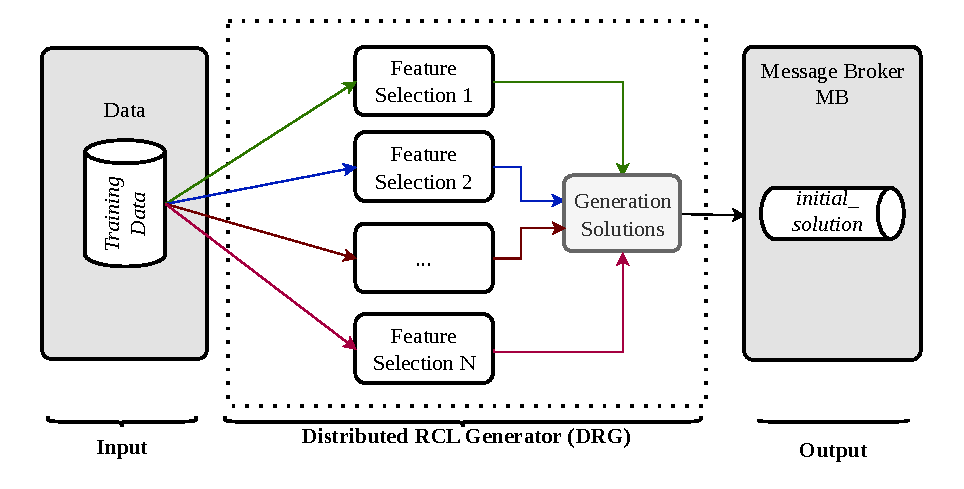
\includegraphics[width=.96\linewidth,height=.82\textheight,keepaspectratio]{fig/gfshield/generic-drg.pdf}
  \caption{Arquitetura genérica da etapa \ac{drg}.}
  \label{fig:drg-generic}
\end{figure}
\end{landscape}

\begin{landscape}
\begin{figure}[p]
  \centering
  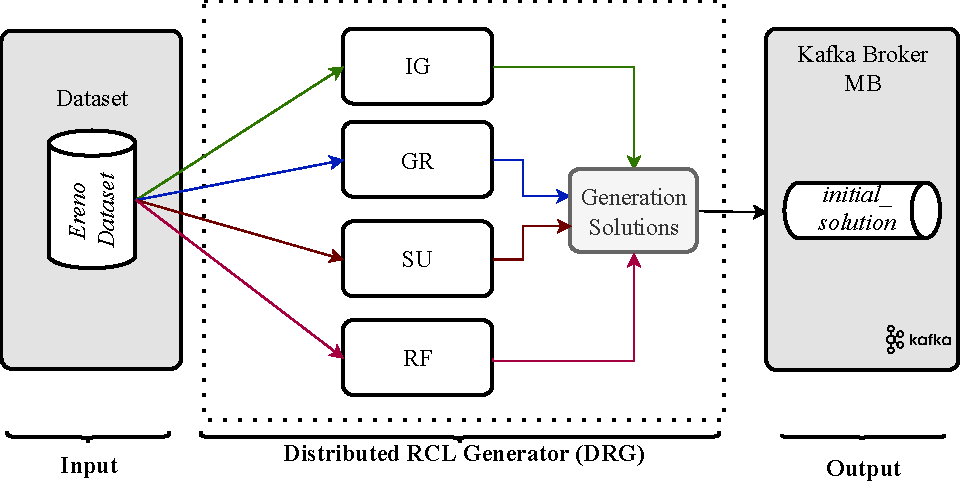
\includegraphics[width=.96\linewidth,height=.82\textheight,keepaspectratio]{fig/gfshield/drg-specific.pdf}
  \caption{Instanciação da etapa \ac{drg} com as quatro métricas implementadas.}
  \label{fig:drg-specific}
\end{figure}
\end{landscape}

Em cada geração, o serviço copia sua RCL e sorteia \texttt{sampleSize} posições uniformemente, sem reposição nessa cópia. Na campanha formal, o gerador é inicializado por \texttt{CAMPAIGN\_RANDOM\_SEED}; o \texttt{seedId} identifica a solução, enquanto \texttt{campaignId}, \texttt{runId}, \texttt{requestId} e a semente numérica preservam a proveniência. O subconjunto é avaliado no treino e na validação reduzidos; o teste reservado não participa da busca. A mensagem publicada preserva subconjunto, RCL, métricas internas e configuração de refinamento.

A Listagem~\ref{lst:drg-pseudocode} apresenta esse comportamento em pseudocódigo. \texttt{metric} identifica um dos quatro ramos. Os parâmetros são mapeados assim:
\begin{itemize}
  \item \texttt{G}: \texttt{maxGenerations};
  \item \texttt{k}: \texttt{rclCutoff};
  \item \texttt{s}: \texttt{sampleSize}.
\end{itemize}

\begin{lstlisting}[caption={Formação da RCL e construção aleatória implementadas no DRG.},label={lst:drg-pseudocode},basicstyle=\ttfamily\small,breaklines=true,columns=fullflexible]
procedure DRG(trainFile, validationFile, metric, G, k, s, classifier,
              neighborhood, enabledSearches, iterationLimits, runSeed)
  train <- readARFF(trainFile); train.class <- lastAttribute
  valid <- readARFF(validationFile); valid.class <- lastAttribute
  rng <- PseudoRandomGenerator(runSeed)

  scored <- empty list
  for each predictor a in train, excluding the class do
    scored.append((metric(train, a), oneBasedIndex(a)))
  end for
  ranking <- sortDescending(scored)
  rcl <- first min(k, size(ranking)) feature identifiers

  for generation <- 1 to G do
    pool <- copy(rcl)
    selected <- empty list
    repeat min(s, size(pool)) times
      p <- UniformInteger(rng, 1, size(pool))
      selected.append(removeAt(pool, p))
    end repeat

    seedId <- randomUUID()
    scores <- trainAndValidate(classifier, train, valid, selected)
    appendServiceMetricsCSV(selected, scores, classifier,
                            trainFile, validationFile)
    publish(INITIAL_SOLUTION_TOPIC,
            {seedId, selected, rcl, scores, metric,
             neighborhood, enabledSearches, iterationLimits})
  end for
end procedure
\end{lstlisting}

\section{Busca Local Distribuída}

Os controladores \ac{vnd} e \ac{rvnd} recebem cada solução inicial e encaminham mensagens aos operadores Bit Flip, \ac{iwss} e \ac{iwssr}. O VND percorre as buscas habilitadas na ordem configurada, compara o melhor resultado do ciclo com sua linha de base e reinicia o ciclo quando ocorre melhora e ainda existe orçamento de despachos. O RVND seleciona aleatoriamente uma busca habilitada a cada passo e continua até o limite de iterações. O uso de VND e da variante randomizada é fundamentado na literatura de vizinhanças variáveis e RVND~\cite{MladenovicHansen1997VNS,DuarteEtAl2018VND,SUBRAMANIAN20101899}; a distribuição desses operadores segue o GDLS-FS~\cite{Silva2023GDLSFS}.

O Bit Flip troca aleatoriamente um atributo do subconjunto por um atributo da lista de candidatos a cada iteração. O IWSS adiciona sequencialmente o primeiro atributo ainda disponível e preserva o melhor subconjunto avaliado. O IWSSR executa o movimento de adição e, para cada posição do subconjunto resultante, avalia a remoção correspondente, conservando a melhor substituição. Esses operadores de vizinhança seguem as avaliações do GRASP-FS~\cite{quincozes2020grasp,quincozes2021performance,quincozes2022extended}. A RCL encaminhada ao DLS ainda contém atributos da solução inicial, mas a campanha canoniza a solução final e rejeita subconjuntos vazios, inválidos ou duplicados. Os operadores treinam no treino, pontuam candidatos na validação e publicam o resultado em \texttt{SOLUTIONS\_TOPIC}. O verificador mantém o maior F1 interno por \texttt{seedId} e publica uma melhora estrita em \texttt{BEST\_SOLUTION\_TOPIC}; isso representa o melhor resultado observado, não certificado global de otimalidade.

\begin{landscape}
\begin{figure}[p]
  \centering
  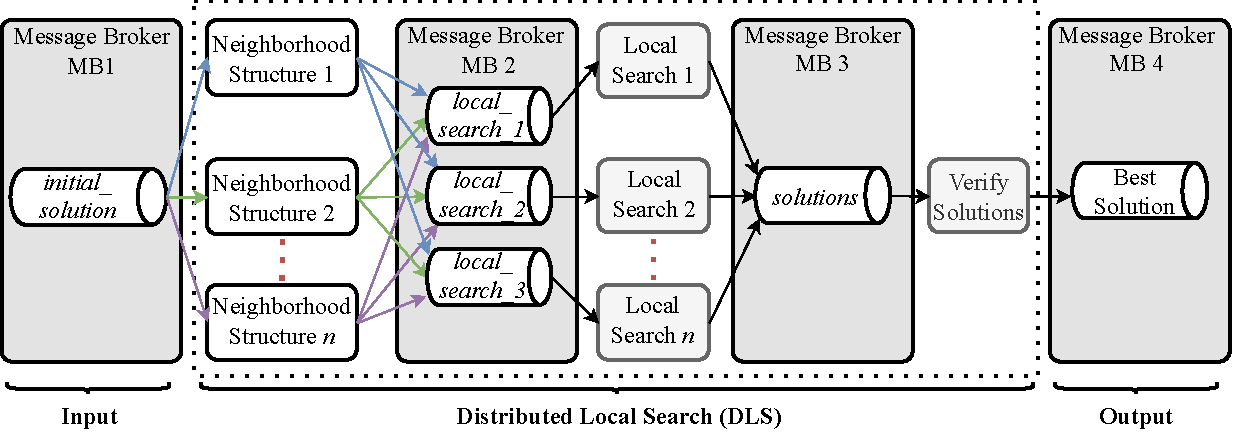
\includegraphics[width=.96\linewidth,height=.82\textheight,keepaspectratio]{fig/gfshield/dls-generic.pdf}
  \caption{Arquitetura genérica da etapa \ac{dls}.}
  \label{fig:dls-generic}
\end{figure}
\end{landscape}

\begin{landscape}
\begin{figure}[p]
  \centering
  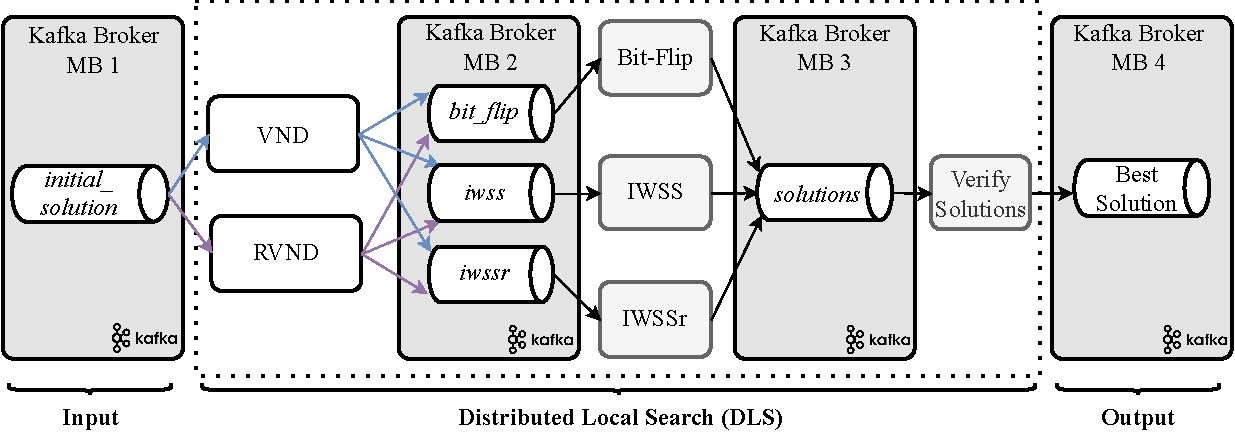
\includegraphics[width=.96\linewidth,height=.82\textheight,keepaspectratio]{fig/gfshield/dls-specific.pdf}
  \caption{Instanciação da etapa \ac{dls} com os controladores e operadores implementados.}
  \label{fig:dls-specific}
\end{figure}
\end{landscape}

A Listagem~\ref{lst:dls-pseudocode} resume a orquestração efetiva. O orçamento do VND é o número configurado de ciclos multiplicado pela quantidade de buscas habilitadas; o RVND usa diretamente o limite de iterações. Os valores padrão dos dois controladores são dez quando a requisição não fornece um limite.

\begin{lstlisting}[caption={Refinamento e verificação distribuídos implementados no DLS.},label={lst:dls-pseudocode},basicstyle=\ttfamily\small,breaklines=true,columns=fullflexible]
on INITIAL_SOLUTION_TOPIC or NEIGHBORHOOD_RESTART_TOPIC receive seed
  best <- seed
  searches <- configured searches or [BIT_FLIP, IWSS, IWSSR]

  if seed.neighborhood = VND then
    dispatchBudget <- maxCycles * size(searches)
    repeat while dispatchBudget remains
      baseline <- best.F1
      for each search in searches in configured order do
        candidate <- dispatchAndReceive(search, best)
        best <- argmaxF1(best, candidate)
        dispatches <- dispatches + 1
      end for
      if best.F1 <= baseline then stop
    end repeat
  else if seed.neighborhood = RVND then
    repeat until maxIterations dispatches
      search <- UniformChoice(searches)
      candidate <- dispatchAndReceive(search, best)
      best <- argmaxF1(best, candidate)
      dispatches <- dispatches + 1
    end repeat
  end if

  for each candidate received by verifier do
    if bestSeen[candidate.seedId] is undefined or
       candidate.F1 > bestSeen[candidate.seedId].F1 then
      bestSeen[candidate.seedId] <- candidate
      publish(BEST_SOLUTION_TOPIC, candidate)
    end if
  end for
end receive
\end{lstlisting}

O protocolo formal inicializa a construção, o Bit Flip e o RVND com a semente numérica da execução e a persiste separadamente do UUID \texttt{seedId}. Isso torna a sequência pseudoaleatória repetível no ambiente versionado; concorrência, ordem de mensagens e plataforma ainda podem introduzir variação, razão pela qual cada resultado preserva também timestamps, comando e artefatos.

\section{Orquestração por Eventos}

O Kafka desacopla produtores e consumidores pelos seguintes grupos de tópicos:
\begin{itemize}
  \item construção: \path{INITIAL_SOLUTION_TOPIC};
  \item operadores: \path{BIT_FLIP_TOPIC}, \path{IWSS_TOPIC} e \path{IWSSR_TOPIC};
  \item coordenação: \path{SOLUTIONS_TOPIC} e \path{NEIGHBORHOOD_RESTART_TOPIC};
  \item progresso monitorado: \path{LOCAL_SEARCH_PROGRESS_TOPIC};
  \item melhor resultado observado: \path{BEST_SOLUTION_TOPIC}.
\end{itemize}
A chave das mensagens de solução é o \texttt{seedId}, quando disponível. Essa separação permite que eventos observados alimentem o monitor~\cite{Kreps2011}.

\begin{landscape}
\begin{figure}[p]
  \centering
  \includegraphics[width=.96\linewidth,height=.82\textheight,keepaspectratio]{fig/gfshield/gfshield-deployment-topology.pdf}
  \caption{Topologia de implantação e fronteiras de execução do \textit{G-FShield}.}
  \label{fig:deployment-topology}
\end{figure}
\end{landscape}

O Kafka é configurado como log de eventos da execução, mas durabilidade potencial não equivale a recuperação demonstrada. A configuração possui criação automática de tópicos, seis partições e fator de replicação um. Não foram medidos perda ou duplicação de mensagens, completude dos eventos, custo da instrumentação, comportamento após reinício, recuperação de consumidor ou reprocessamento. Por isso, resiliência e tolerância a falhas permanecem objetivos de projeto.

\section{Telemetria Persistida e Camada Web}

Observabilidade, neste trabalho, significa a possibilidade de inspecionar o estado externo registrado da execução. Não significa explicar causalmente as decisões do classificador. O monitor da \ac{api} consome cinco tópicos de interesse: solução inicial, reinício de vizinhança, progresso de busca local, solução refinada e melhor solução. Cada evento persistido contém tipo, conteúdo JSON e instante de ingestão pelo backend, além de tópico, estágio, estado, \texttt{seedId}, \texttt{requestId}, partição e \textit{offset} quando disponíveis. Uma impressão digital evita inserir novamente o mesmo evento observado. Na campanha formal, \texttt{campaignId}, \texttt{runId}, \texttt{requestId}, \texttt{seedId}, timestamp UTC do produtor e tempo monotônico são propagados nos objetos experimentais.

O PostgreSQL mantém três níveis principais: o lançamento solicitado, a execução corrente por \texttt{seedId} e o histórico de eventos associado. O estado da execução inclui algoritmo da RCL, classificador, busca local, vizinhança, arquivos, iterações, F1, acurácia, precisão, revocação, CPU, memória, tempo e conjuntos de atributos. Modelos de leitura materializados agregam tópicos, algoritmos, recursos e intervalos da linha do tempo. O Redis armazena temporariamente respostas consultadas com frequência; a fonte persistente é o PostgreSQL.

Os serviços Java também escrevem CSVs por componente no volume \texttt{/metrics}. Esses arquivos contêm subconjunto, F1, acurácia, precisão, revocação, tempo, CPU, memória, classificador e nomes dos arquivos. Como os CSVs atuais não registram o \texttt{seedId}, sua correlação direta com o histórico web não deve ser presumida. Os \textit{logs} Java e Node são emitidos em \textit{stdout}; o Compose não configura armazenamento de logs, política de retenção ou coletor como Loki/ELK. Portanto, eventos e métricas são persistidos pela aplicação, mas a persistência de logs depende do runtime externo e não foi demonstrada.

A combinação de identificadores, eventos e \textit{timestamps} permite reconstruir a linha do tempo que chegou ao monitor e comparar estados de uma mesma semente. Ela não garante que todos os eventos produzidos foram capturados. Na campanha formal, a semente numérica, o \texttt{runId} e os checksums complementam essa telemetria; completude do monitor e reprodutibilidade em outro hardware continuam limitadas.

\begin{figure}[p]
  \centering
  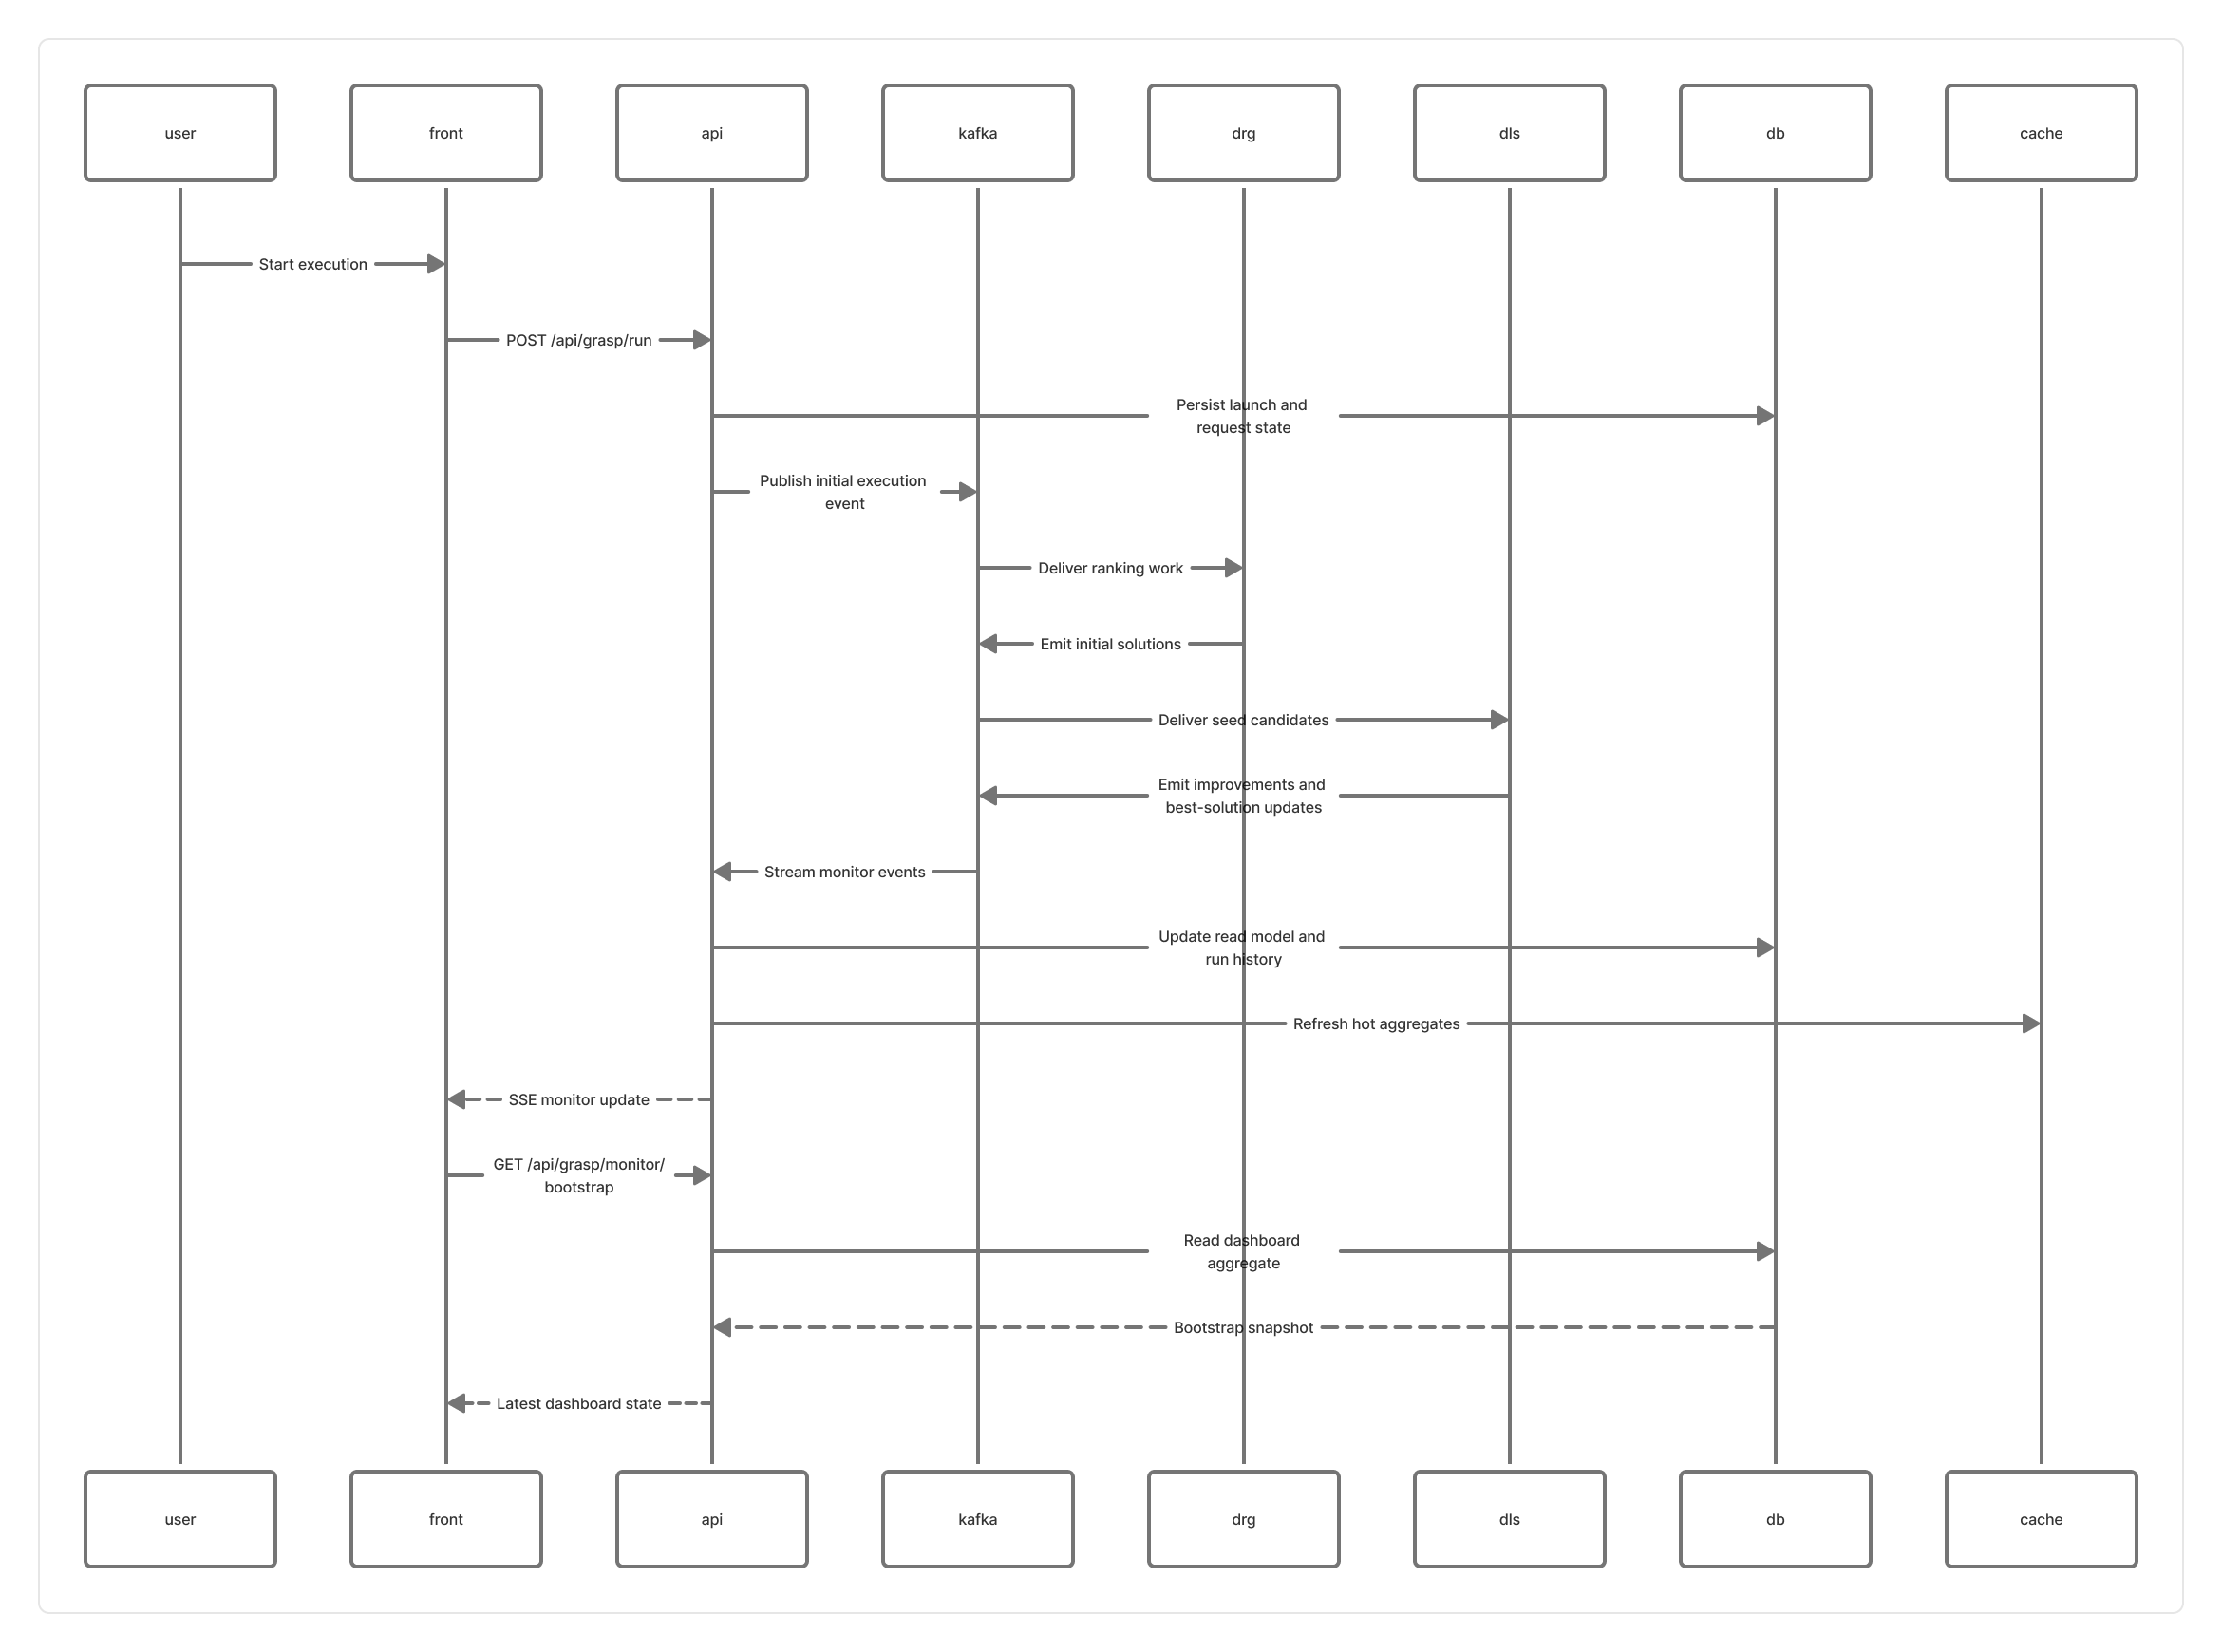
\includegraphics[width=\linewidth,height=.74\textheight,keepaspectratio]{fig/gfshield/g-fshield-execution-lifecycle.png}
  \caption{Ciclo de execução do \textit{G-FShield}, da solicitação aos estados apresentados na interface.}
  \label{fig:execution-lifecycle}
\end{figure}

\begin{figure}[p]
  \centering
  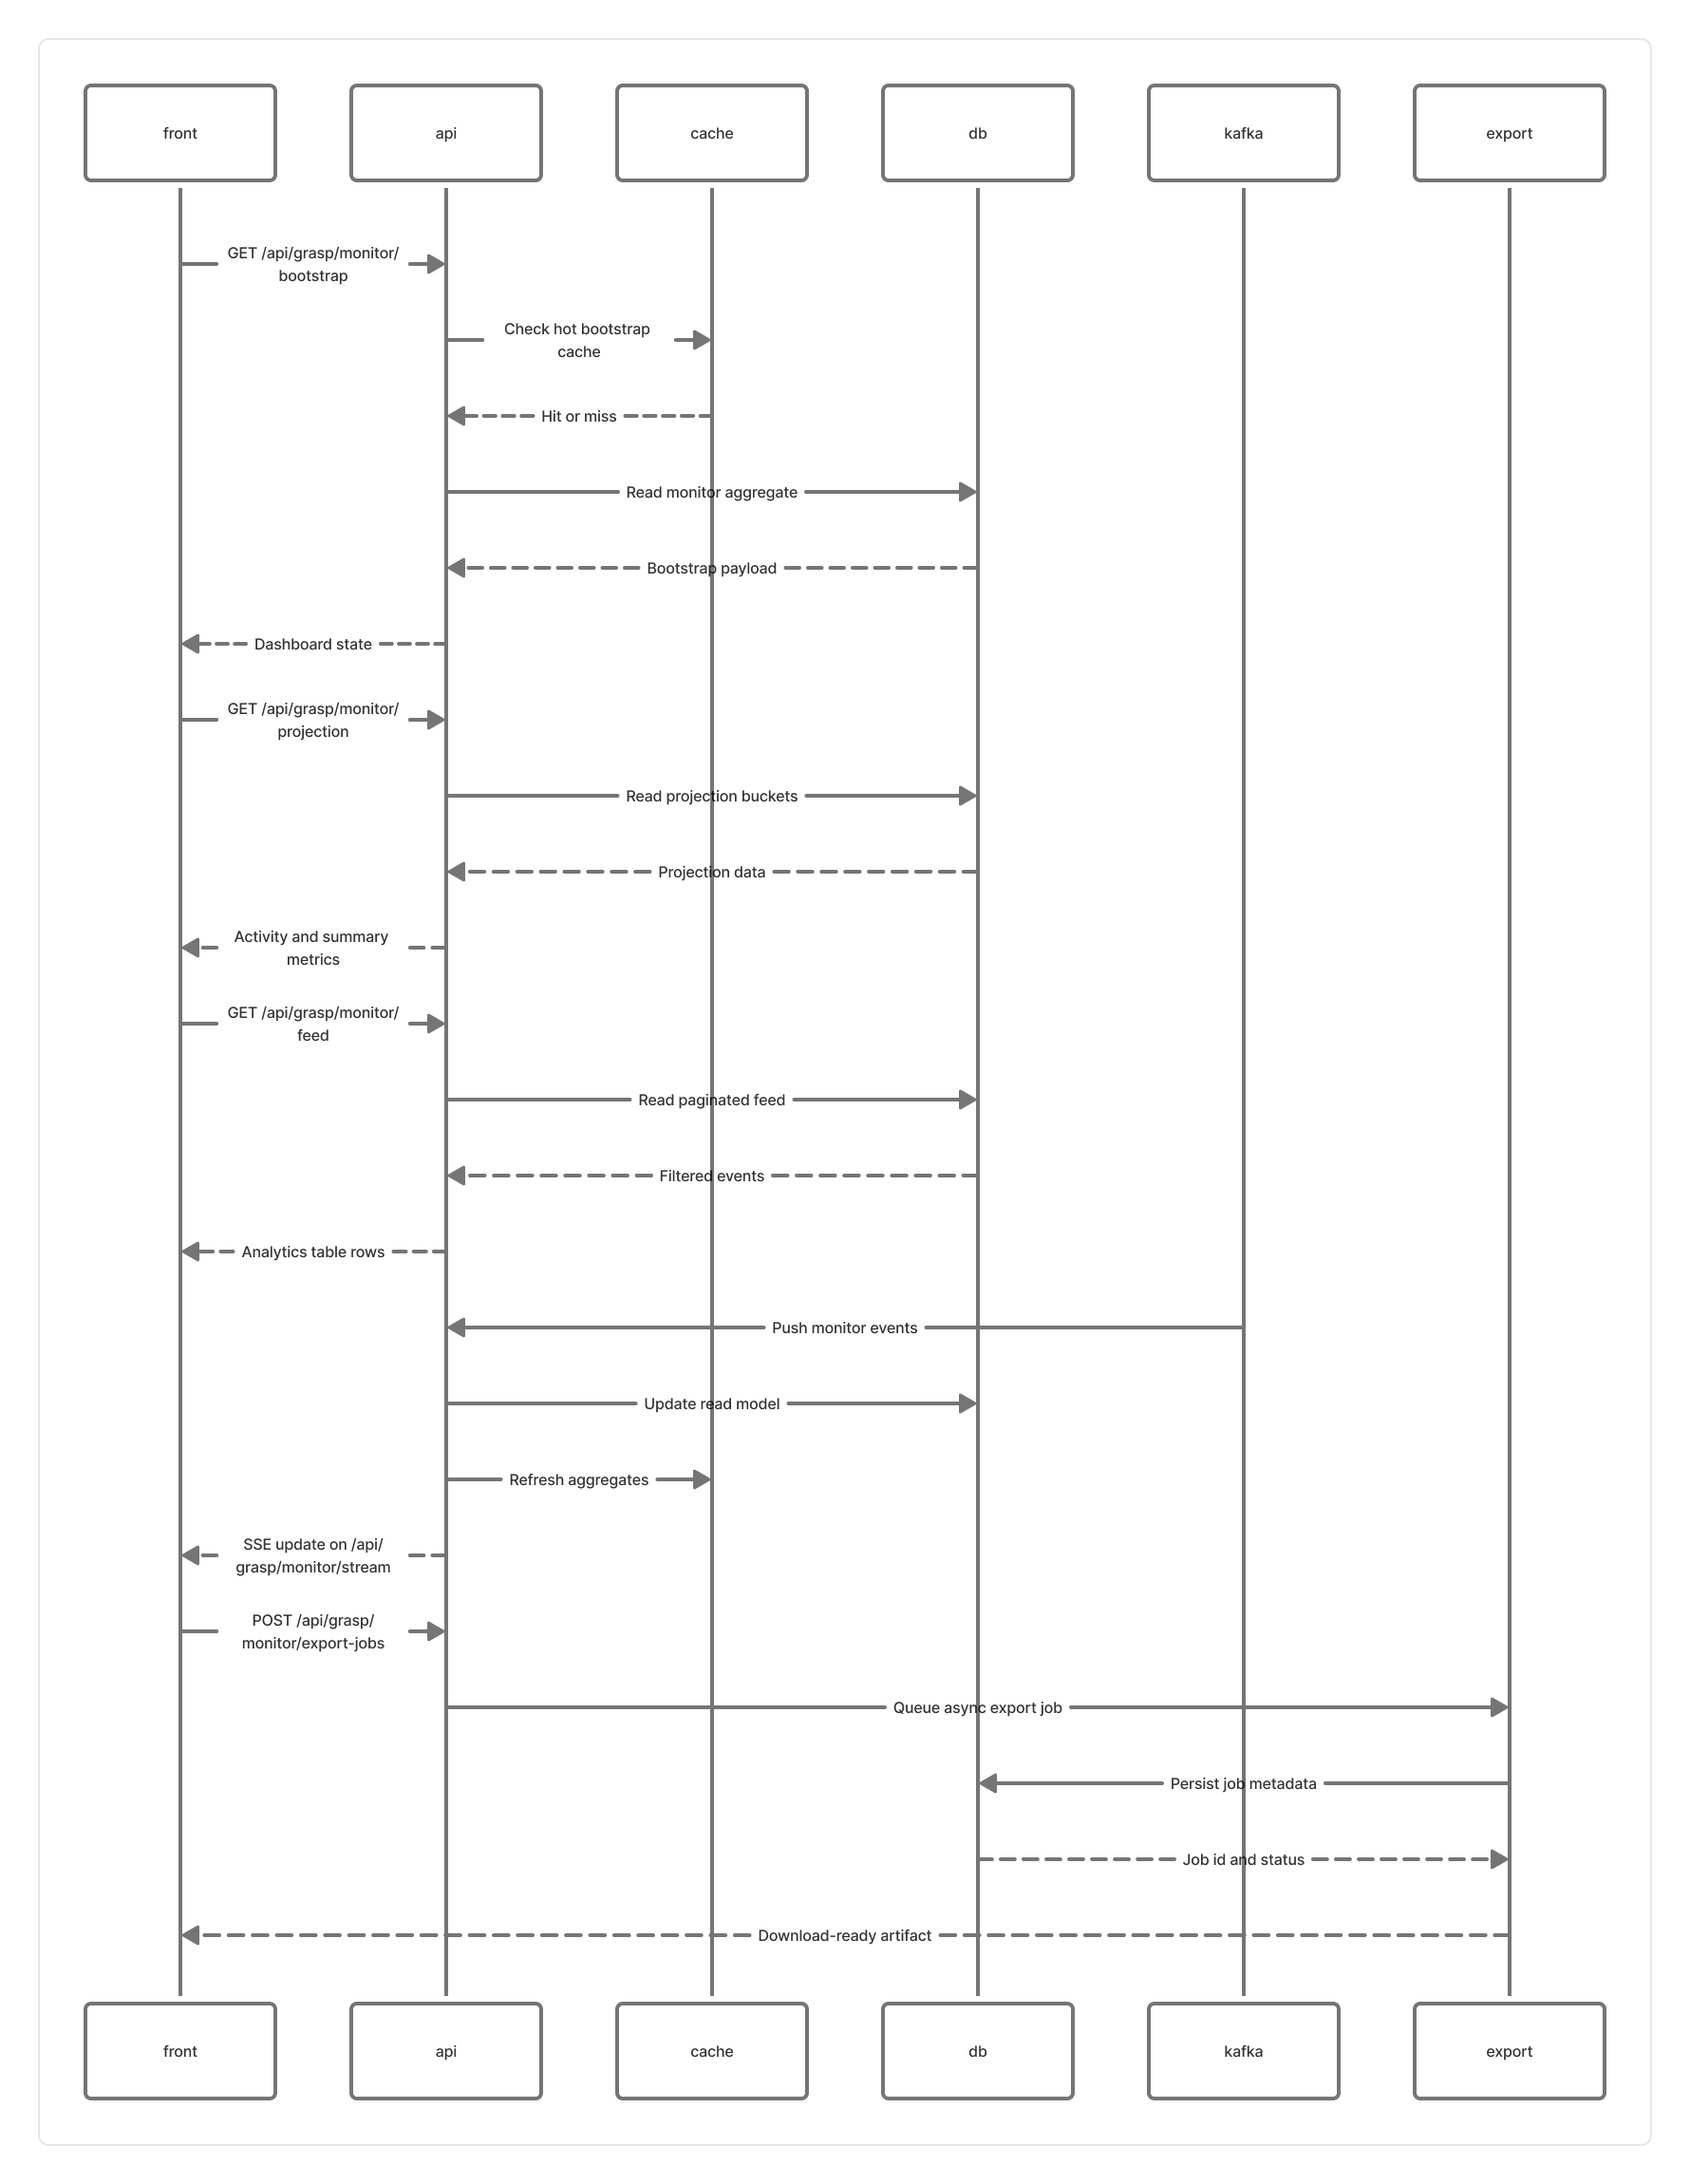
\includegraphics[width=\linewidth,height=.82\textheight,keepaspectratio]{fig/gfshield/g-fshield-monitoring-pipeline.png}
  \caption{Pipeline de ingestão, persistência e apresentação da telemetria observada.}
  \label{fig:monitoring-pipeline}
\end{figure}

A implementação web usa React e Vite no cliente; Express e Swagger na \ac{api}; PostgreSQL para persistência; e Redis como \textit{cache} opcional. A interface consulta resumos, eventos paginados, linhas do tempo e exportações CSV ou JSON. Essas tecnologias descrevem a implementação; por si só, não comprovam produtividade, estabilidade, responsividade ou desempenho.

\begin{figure}[p]
  \centering
  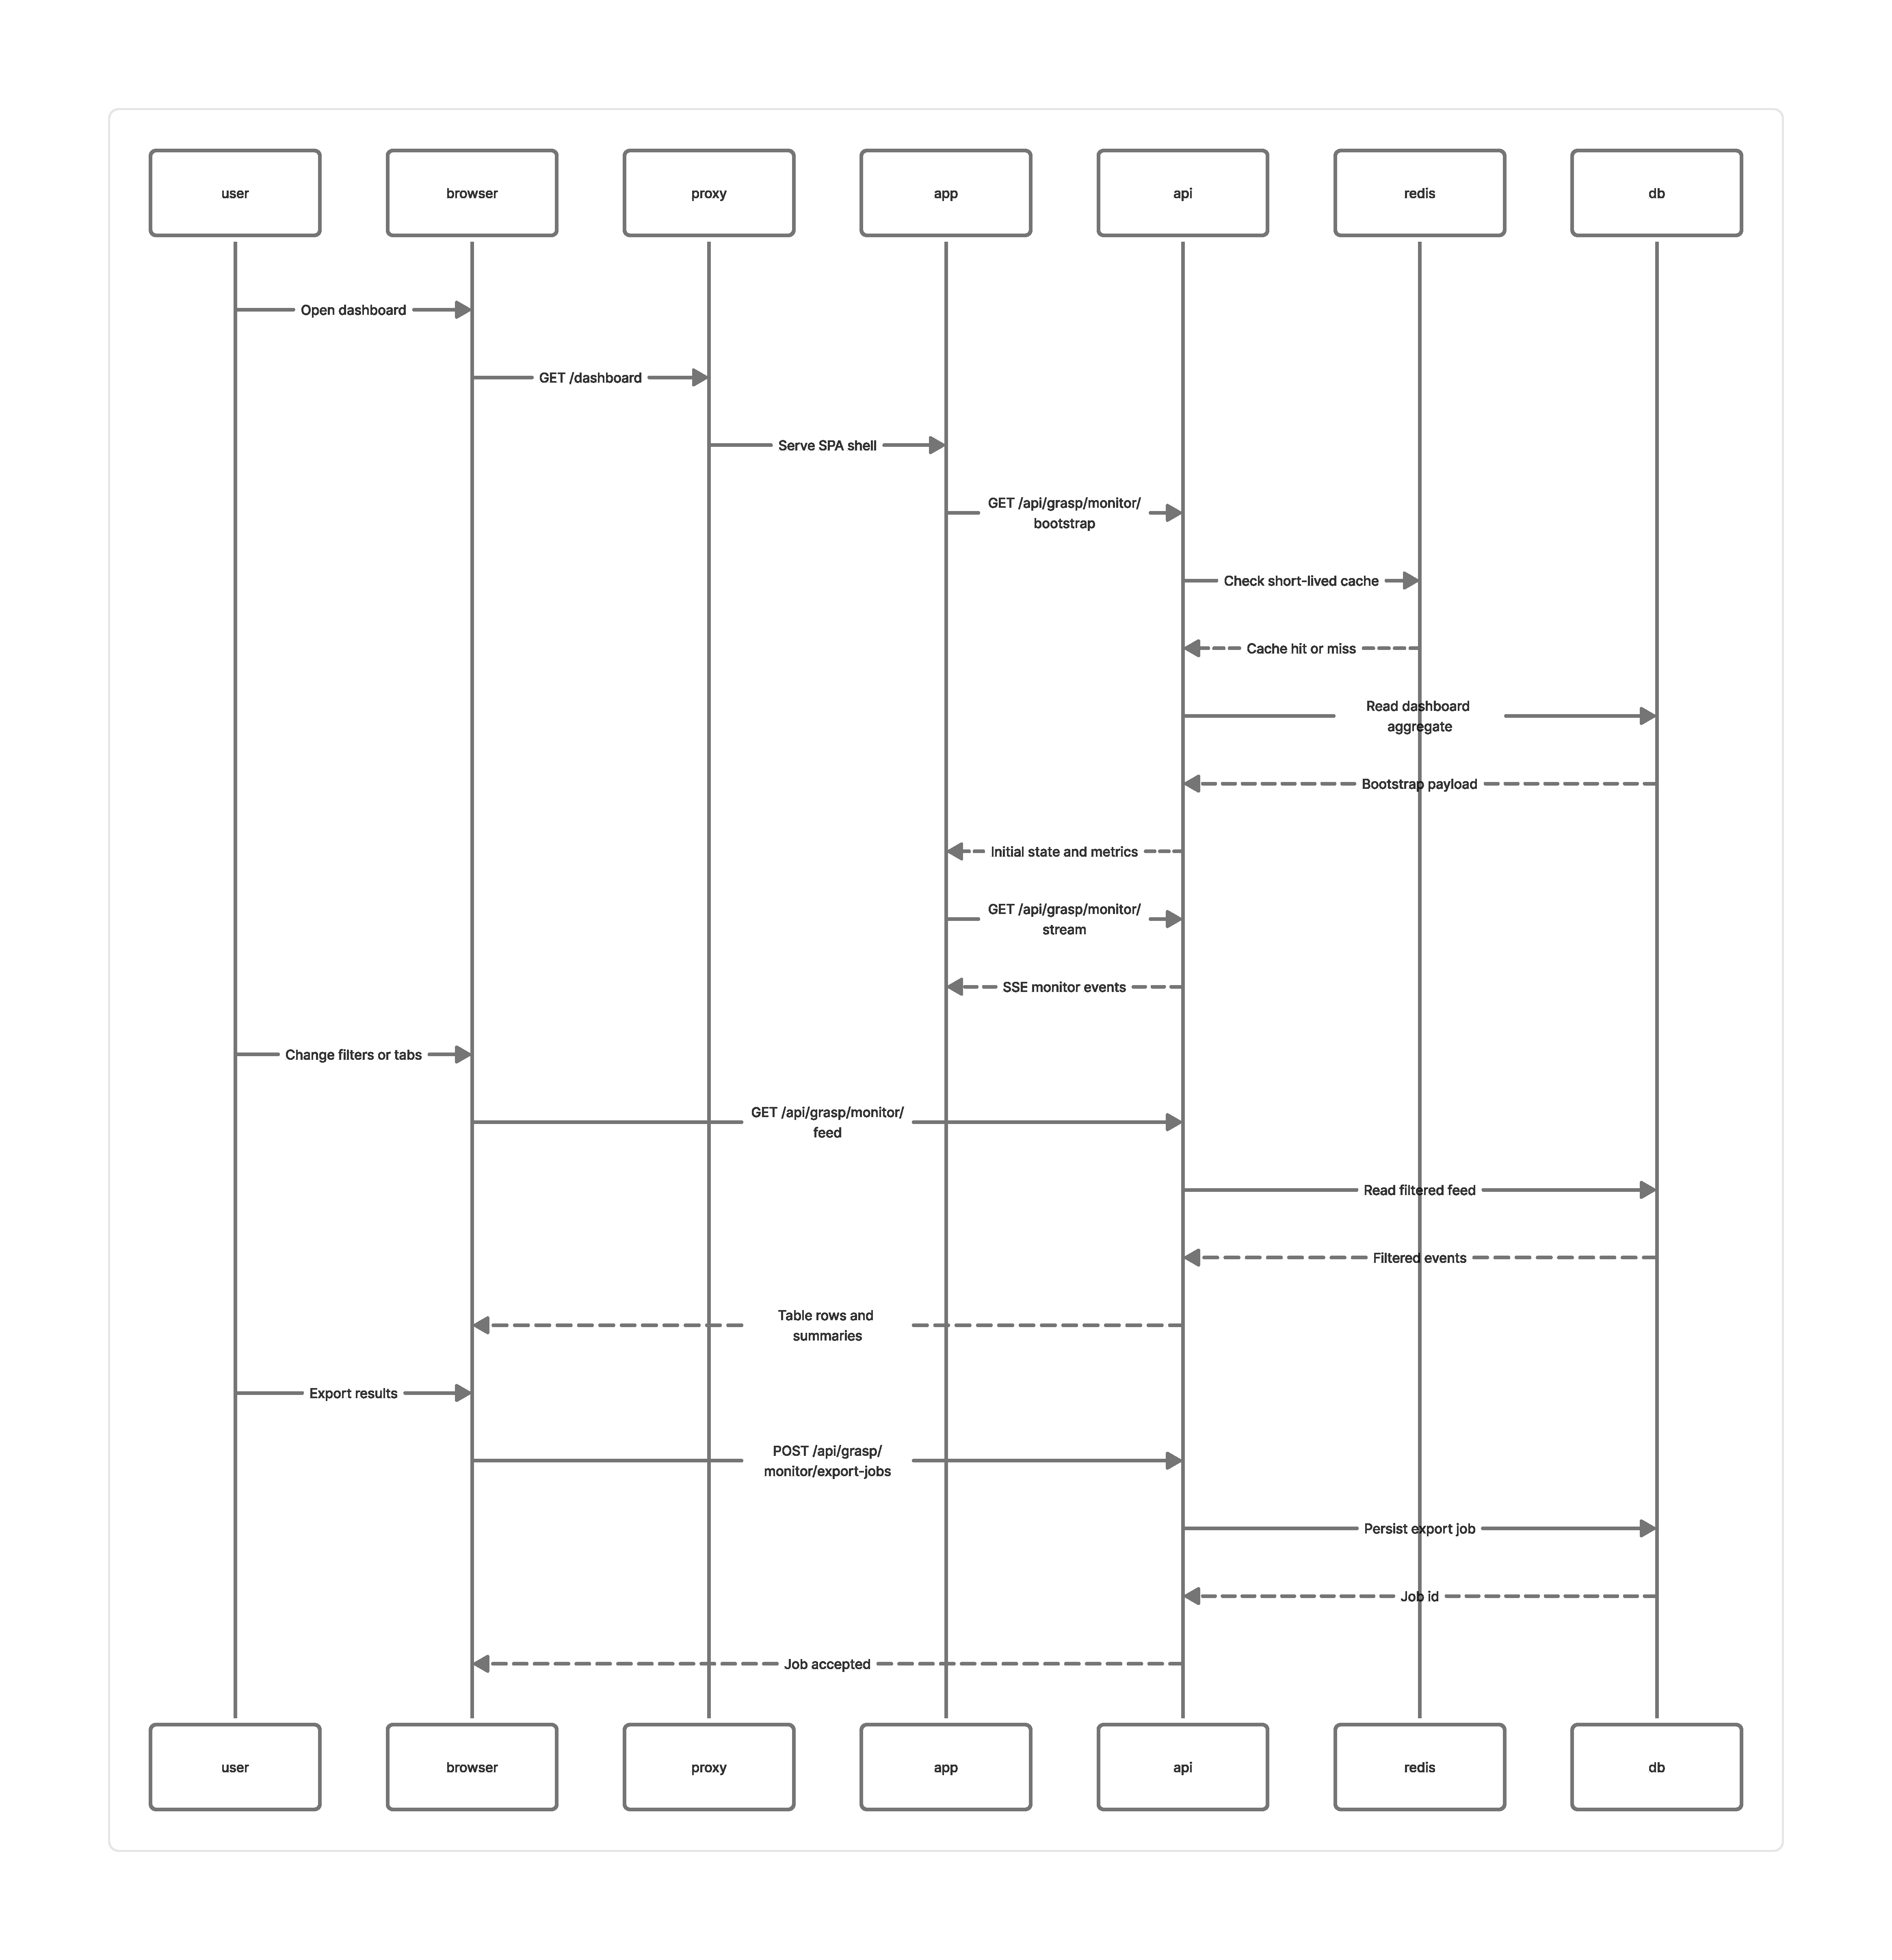
\includegraphics[width=\linewidth,height=.82\textheight,keepaspectratio]{fig/gfshield/gfshield-front-flow.pdf}
  \caption{Fluxo funcional do cliente web e de suas consultas à \ac{api}.}
  \label{fig:front-flow}
\end{figure}

\begin{landscape}
\begin{figure}[p]
  \centering
  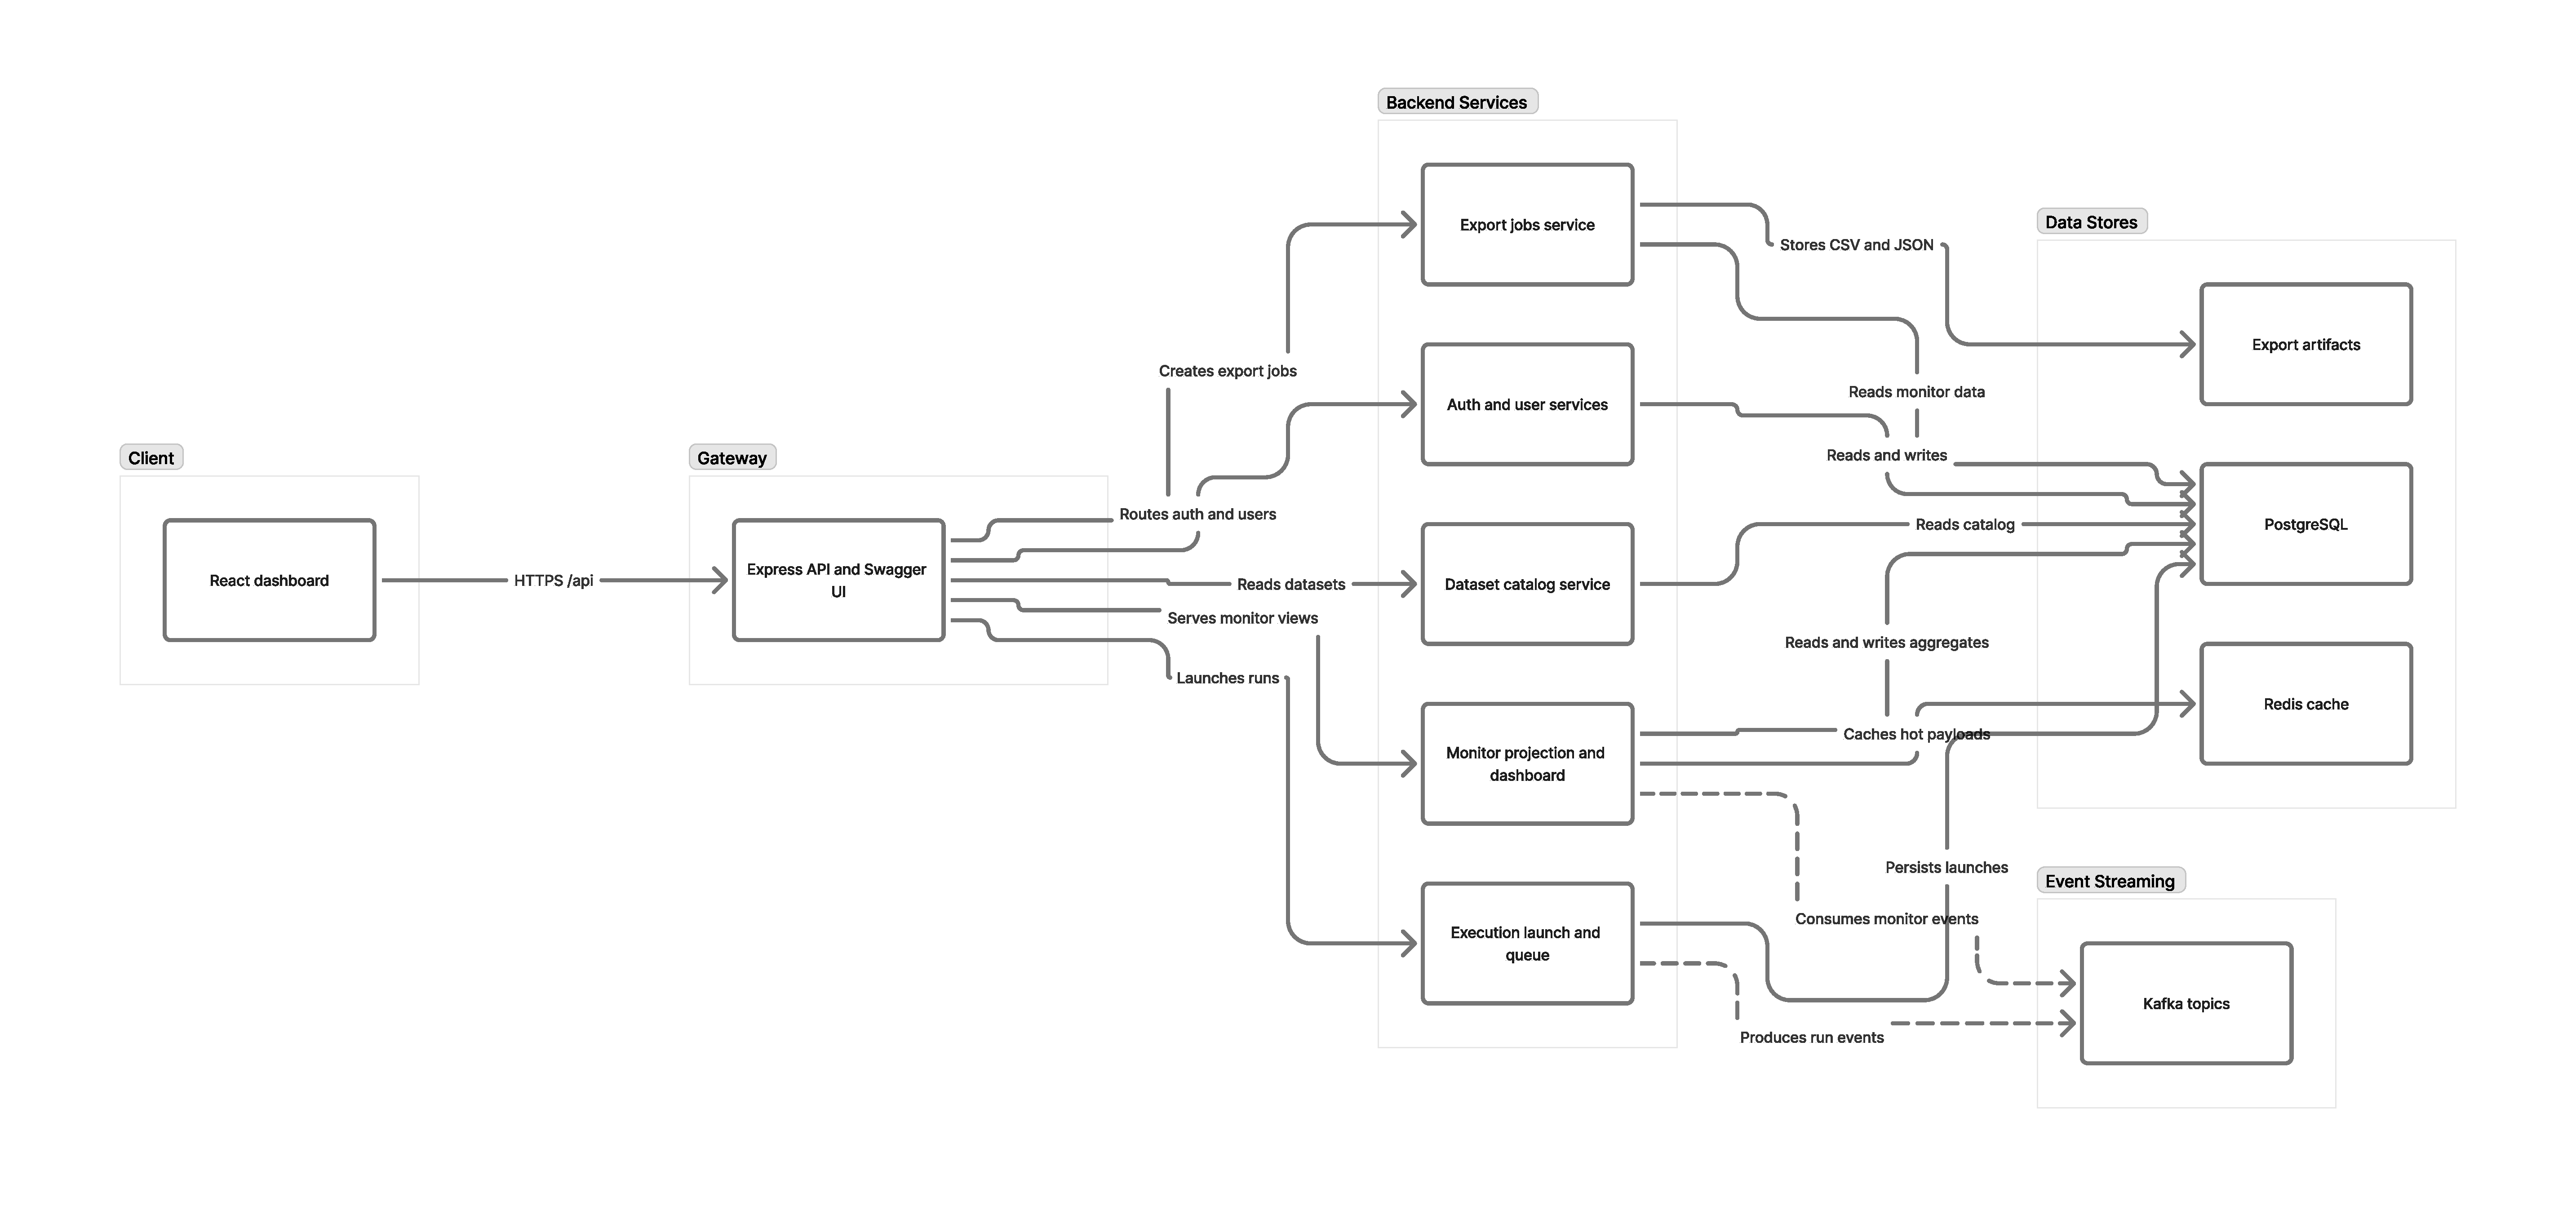
\includegraphics[width=.96\linewidth,height=.82\textheight,keepaspectratio]{fig/gfshield/gfshield-backend-architecture.pdf}
  \caption{Serviços do backend, armazenamentos e integração com a mensageria.}
  \label{fig:backend-architecture}
\end{figure}
\end{landscape}

As Figuras~\ref{fig:execution-lifecycle} a~\ref{fig:backend-architecture} complementam a visão abstrata com os fluxos implementados. As capturas da interface, a documentação da \ac{api} e os diagramas de apoio encontram-se nos Apêndices~\ref{app:frontend},~\ref{app:video-docs} e~\ref{app:diagrams}.

\section{Configuração de Referência e Reprodutibilidade}

A Tabela~\ref{tab:container-resources} registra a configuração local definida por três arquivos:
\begin{itemize}
  \item \path{docker-compose.yml};
  \item \path{docker-compose.local.yml};
  \item \path{webservice/api/docker-compose.db.yml}.
\end{itemize}
Os valores são limites por contêiner. O \textit{preset} de servidor aumenta parte desses limites e, portanto, não deve ser misturado a uma comparação experimental sem registro explícito.

\begin{table}[!htb]
  \centering
  \scriptsize
  \caption{Recursos e concorrência da configuração local de referência.}
  \label{tab:container-resources}
  \begin{tabularx}{\linewidth}{@{}Xc c c X@{}}
    \toprule
    \textbf{Grupo de serviços} & \textbf{Qtd.} & \textbf{CPU/unid.} & \textbf{RAM/unid.} & \textbf{Concorrência/configuração} \\
    \midrule
    DRG: IG, GR, SU e ReliefF & 4 & 1,50 & 1536 MB & \textit{pool} assíncrono: núcleo 2, máximo 4, fila 80 \\
    DLS: Bit Flip, IWSS e IWSSR & 3 & 1,00 & 1536 MB & um consumidor Kafka por serviço \\
    VND, RVND e verificador & 3 & 0,75 & 768 MB & um consumidor Kafka por serviço \\
    Kafka & 1 & 1,00 & 1024 MB & seis partições; replicação 1 \\
    ZooKeeper & 1 & 0,50 & 256 MB & porta de cliente 2181 \\
    Kafbat UI & 1 & 0,50 & 512 MB & cliente do Kafka interno \\
    PostgreSQL & 1 & 0,50 & 512 MB & configuração do banco local \\
    Redis & 1 & 0,25 & 256 MB & persistência AOF e \textit{snapshot} configurados \\
    \bottomrule
  \end{tabularx}
\end{table}

O hospedeiro indicado como servidor de execução foi inspecionado em 25 de agosto de 2026. A máquina, identificada pelo sistema como \texttt{mc2-server-01}, possui dois processadores Intel Xeon E5-2620 v4 a 2,10 GHz, com oito núcleos e duas \textit{threads} por núcleo em cada soquete, totalizando 16 núcleos físicos e 32 processadores lógicos em dois nós NUMA. O Docker detectou 67.447.271.424 bytes de memória (64.322,73 MiB; aproximadamente 62,8 GiB), e o sistema tinha 8 GiB de \textit{swap}. O ambiente usa Ubuntu 18.04.6 LTS, arquitetura x86-64 e \textit{kernel} Linux 4.15.0-213-generic. Foram observados Docker Engine/cliente 24.0.2, API 1.43, \textit{storage driver} \texttt{overlay2}, \textit{cgroup driver} \texttt{cgroupfs}, \texttt{docker compose} 2.18.1 e o executável \texttt{docker-compose} 2.30.3.

Os rótulos do Docker ligavam os serviços em execução ao projeto \texttt{g-fshield} e à sobreposição de \path{docker-compose.yml} com \path{docker-compose.server.yml}. A Tabela~\ref{tab:server-container-resources} registra os limites efetivos observados. Havia uma instância de cada serviço; não havia modo Swarm nem replicação adicional de contêiner. PostgreSQL e Redis pertenciam a uma segunda composição, formada por \path{webservice/api/docker-compose.db.yml} e \path{webservice/api/docker-compose.db.server.yml}. A \ac{api} e o cliente web não apareciam na lista de contêineres, de modo que não se atribui a eles um limite observado.

Na raiz do repositório, os comandos correspondentes aos arquivos registrados nos rótulos são:
\begin{lstlisting}[basicstyle=\ttfamily\footnotesize,breaklines=true,columns=fullflexible]
docker compose -f docker-compose.yml -f docker-compose.server.yml up -d
docker compose -f webservice/api/docker-compose.db.yml -f webservice/api/docker-compose.db.server.yml up -d
\end{lstlisting}
Esses comandos reconstroem a composição observada; não substituem um histórico de terminal ou manifesto que confirme as opções usadas na campanha.

\begin{table}[!htb]
  \centering
  \scriptsize
  \caption{Limites efetivos no servidor inspecionado.}
  \label{tab:server-container-resources}
  \begin{tabularx}{\linewidth}{@{}Xc c c X@{}}
    \toprule
    \textbf{Grupo de serviços} & \textbf{Qtd.} & \textbf{CPU/unid.} & \textbf{RAM/unid.} & \textbf{Concorrência/configuração} \\
    \midrule
    DRG: IG, GR, SU e ReliefF & 4 & 2,00 & 2048 MB & \textit{pool}: núcleo 3, máximo 6, fila 150 \\
    DLS: Bit Flip, IWSS e IWSSR & 3 & 1,50 & 2048 MB & um consumidor Kafka por serviço \\
    VND, RVND e verificador & 3 & 1,00 & 1024 MB & um consumidor Kafka por serviço \\
    Kafka & 1 & 2,00 & 2048 MB & seis partições; replicação 1 \\
    ZooKeeper & 1 & 0,75 & 512 MB & uma instância \\
    Kafbat UI & 1 & 1,00 & 2048 MB & uma instância \\
    PostgreSQL & 1 & 1,00 & 1024 MB & uma instância \\
    Redis & 1 & 0,25 & 256 MB & uma instância \\
    \bottomrule
  \end{tabularx}
\end{table}

O diretório \path{/home/idscps/nicolas/graspy2} forneceu a implementação do Monólito~1. O diretório \path{/home/idscps/nicolas/Graspy} forneceu a do Monólito~2. Para a campanha formal, ambos foram reconstruídos em imagens versionadas e executados como um único contêiner por braço sob o mesmo teto agregado. O Monólito~1 ordena atributos por Gain Ratio, constrói um subconjunto de cinco a partir de corte 30 e aplica Bit-Flip por até 100 iterações locais. O Monólito~2 usa Gain Ratio, constrói cinco atributos a partir de RCL de tamanho 30 e aplica IWSS sob VND por até 100 iterações. Ambos recebem as mesmas divisões imutáveis de treino, validação e teste, sementes 42--49, limite de 3.000 s, máximo de 500 melhorias aceitas e melhora mínima de 0,0001.

Durante a busca formal, os dois monólitos e o G-FShield usam Weka J48 e F1 macro na validação. A solução de melhor validação é então avaliada uma única vez no teste. Essa adaptação elimina as diferenças históricas de classificador, função objetivo e escala das métricas, mas preserva algoritmos comparadores diferentes: GR--BF no Monólito~1, GR--IWSS no Monólito~2 e as 24 combinações de ranking, controlador e operador no G-FShield. Por isso, a campanha compara soluções completas, mas não isola causalmente apenas o efeito da distribuição.

Os quatro serviços DRG expõem as portas 8086--8089; Bit Flip, IWSS, IWSSR e o verificador usam 8082--8085; RVND e VND usam 8090 e 8091. Kafka expõe 19092, ZooKeeper 2181, JMX 9999 e Kafbat UI 8080. A \ac{api}, o cliente web, PostgreSQL e Redis usam, por padrão, 4000, 3000, 5432 e 6379. Os conjuntos de dados e os CSVs são volumes vinculados aos diretórios \texttt{datasets/} e \texttt{metrics/}; PostgreSQL e Redis usam volumes nomeados.

As imagens Java são construídas com Maven 3.9.4 e Eclipse Temurin 17 e executadas no Temurin 17 JRE. A maioria dos módulos de avaliação declara Weka 3.8.0; o \texttt{pom.xml} do serviço SU contém declarações duplicadas para 3.8.6 e 3.8.0, de modo que a árvore de dependências resolvida deve ser arquivada. Os DRG usam Spring Boot 3.0.0 e os DLS, Spring Boot 2.7.5. A infraestrutura fixa as seguintes imagens:
\begin{itemize}
  \item \path{confluentinc/cp-kafka:7.4.0};
  \item \path{confluentinc/cp-zookeeper:7.4.0};
  \item \path{ghcr.io/kafbat/kafka-ui:v1.4.2};
  \item \path{postgres:14};
  \item \path{redis:7-alpine}.
\end{itemize}
O modo opcional que executa a camada web em contêiner usa \texttt{node:24}; o projeto declara Express 4.21.1, React 18.2.0 e Vite 8.0.3. Os arquivos Compose não impõem limites de CPU e RAM à \ac{api} e ao cliente web iniciados pelos scripts; esses limites também precisam ser fixados em uma reprodução de desempenho.

\subsection{Manifesto da campanha formal}

O identificador da campanha formal é \texttt{gfshield-10d-2026-v1}. Sua \textit{tag} é \texttt{experiment-10d-v1}, e o \textit{commit} de lançamento é \texttt{66565b865a7b}. As imagens foram construídas do \textit{commit} \texttt{b38eff3ed9c1}; o manifesto preserva o ID SHA-256 de cada imagem local e os \textit{digests} de Kafka 7.4.0 e ZooKeeper 7.4.0. O manifesto, o Compose resolvido e a proveniência do hospedeiro possuem hashes próprios. Cada execução também arquiva comando, Compose resolvido, logs, métricas, telemetria, resultado final e um manifesto de checksums.

O arquivo \path{experiments/10-day-campaign/frozen-compose.yaml} fixa os serviços usados no protocolo. Cada configuração distribuída inicia um gerador de RCL, VND ou RVND, os três operadores BF/IWSS/IWSSR, o verificador, Kafka e ZooKeeper. Há um consumidor por serviço e uma partição lógica de execução; Kafka usa seis partições, fator de replicação um e criação automática de tópicos. Os serviços Java usam Temurin 17; o avaliador comum usa Weka 3.8.6. Os monólitos são imagens separadas, derivadas de \path{graspy2} e \path{Graspy}. Todos os braços usam \texttt{--cpuset-cpus 8-15}, \texttt{--cpuset-mems 1}, teto agregado de oito CPUs e 16~GiB. O kernel do hospedeiro não oferece contabilização de \textit{swap} ao Docker; o limite de memória foi aplicado, mas um limite de \textit{swap} separado não pôde ser verificado.

Os dados são montados somente para leitura em \path{/data} ou \path{/datasets}; resultados, logs e métricas usam volumes vinculados específicos de cada \texttt{run\_id}. As portas dos geradores são publicadas apenas em \texttt{127.0.0.1} durante a execução; Kafka e os demais serviços comunicam-se na rede interna da composição. A camada web não integra o caminho medido da campanha.

O lançamento durável foi realizado no servidor por:

\begin{lstlisting}[basicstyle=\ttfamily\footnotesize,breaklines=true,columns=fullflexible]
python3 experiments/10-day-campaign/campaign_supervisor.py \
  --manifest experiments/10-day-campaign/manifest.yaml \
  --state experiments/10-day-campaign/state/campaign-state.json \
  --supervisor-state experiments/10-day-campaign/state/supervisor-state.json \
  --log experiments/10-day-campaign/logs/campaign-supervisor.log \
  --output-root experiments/10-day-campaign/results
\end{lstlisting}

O supervisor preserva o prazo absoluto, verifica espaço livre, encerra grupos de processos e limita reinícios. Na execução reportada, ele não reiniciou. A campanha produziu 216 resultados válidos para 27 braços e oito sementes, além de 12 tentativas inválidas preservadas e repetidas. O repositório contém o analisador \path{experiments/10-day-campaign/analyze_results.py}, que verifica checksums, normaliza as métricas e recria tabelas e figuras. Reproduzir os resultados ainda depende de acesso às imagens ou de reconstruí-las no \textit{commit} registrado, ao corpus com os hashes indicados e a um hospedeiro compatível; frequências dinâmicas de CPU, contêineres externos e limitações do hardware físico não são eliminados pela conteinerização.

\section{Síntese}

O \textit{G-FShield} integra ramos independentes de construção GRASP-FS, controladores e operadores de busca local, mensageria e verificação de melhores resultados observados. Uma camada web consulta dados mantidos em armazenamento persistente. O contrato de entrada, o pseudocódigo, o manifesto e a configuração dos contêineres delimitam implementação e campanha. A arquitetura oferece desacoplamento, inspeção e evolução; a campanha estabelece rastreabilidade experimental, enquanto escalabilidade, tolerância a falhas e portabilidade entre hospedeiros permanecem propriedades a avaliar.
